\documentclass[
10pt, % Main document font size
a4paper, % Paper type, use 'letterpaper' for US Letter paper
oneside, % One page layout (no page indentation)
%twoside, % Two page layout (page indentation for binding and different headers)
headinclude,footinclude, % Extra spacing for the header and footer
BCOR5mm, % Binding correction
]{scrartcl}
%%%%%%%%%%%%%%%%%%%%%%%%%%%%%%%%%%%%%%%%%
% Arsclassica Article
% Structure Specification File
%
% This file has been downloaded from:
% http://www.LaTeXTemplates.com
%
% Original author:
% Lorenzo Pantieri (http://www.lorenzopantieri.net) with extensive modifications by:
% Vel (vel@latextemplates.com)
%
% License:
% CC BY-NC-SA 3.0 (http://creativecommons.org/licenses/by-nc-sa/3.0/)
%
%%%%%%%%%%%%%%%%%%%%%%%%%%%%%%%%%%%%%%%%%

%----------------------------------------------------------------------------------------
%	REQUIRED PACKAGES
%----------------------------------------------------------------------------------------

\usepackage[
nochapters, % Turn off chapters since this is an article        
beramono, % Use the Bera Mono font for monospaced text (\texttt)
eulermath,% Use the Euler font for mathematics
pdfspacing, % Makes use of pdftex’ letter spacing capabilities via the microtype package
dottedtoc % Dotted lines leading to the page numbers in the table of contents
]{classicthesis} % The layout is based on the Classic Thesis style

\usepackage{arsclassica} % Modifies the Classic Thesis package
\usepackage{ulem}
\usepackage{graphicx}
\usepackage{float}
\usepackage{algorithm2e}
\usepackage[export]{adjustbox}
\usepackage[utf8]{inputenc}  
\usepackage[english,frenchb]{babel} 
\usepackage[T1]{fontenc} % Required for accented characters
\usepackage{multicol}
\usepackage{graphicx} % Required for including images
\graphicspath{{Figures/}} % Set the default folder for images

\usepackage{enumitem} % Required for manipulating the whitespace between and within lists

\usepackage{lipsum} % Used for inserting dummy 'Lorem ipsum' text into the template


\expandafter\def\csname ver@subfig.sty\endcsname{}


\usepackage{svg}
\usepackage{hyperref}

\usepackage{amsmath,amssymb,amsthm} % For including math equations, theorems, symbols, etc

\usepackage{varioref} % More descriptive referencing

%----------------------------------------------------------------------------------------
%	THEOREM STYLES
%---------------------------------------------------------------------------------------

\theoremstyle{definition} % Define theorem styles here based on the definition style (used for definitions and examples)
\newtheorem{definition}{Definition}

\theoremstyle{plain} % Define theorem styles here based on the plain style (used for theorems, lemmas, propositions)
\newtheorem*{remark}{Remark}
\newtheorem{theorem}{Theorème}
\newtheorem{lemma}[theorem]{Lemme}
\newtheorem{proposition}[theorem]{Proposition}

\theoremstyle{remark} % Define theorem styles here based on the remark style (used for remarks and notes)

%----------------------------------------------------------------------------------------
%	HYPERLINKS
%---------------------------------------------------------------------------------------

\hypersetup{
%draft, % Uncomment to remove all links (useful for printing in black and white)
colorlinks=true, breaklinks=true, bookmarks=true,bookmarksnumbered,
urlcolor=webbrown, linkcolor=RoyalBlue, citecolor=webgreen, % Link colors
pdftitle={}, % PDF title
pdfauthor={\textcopyright}, % PDF Author
pdfsubject={}, % PDF Subject
pdfkeywords={}, % PDF Keywords
pdfcreator={pdfLaTeX}, % PDF Creator
pdfproducer={LaTeX with hyperref and ClassicThesis} % PDF producer
}

\hyphenation{Fortran hy-phen-ation} 

\title{\normalfont{FTML Exercices 5}\\
} 
\author{\spacedlowsmallcaps{}
} 
\date{\today}
\begin{document}
\renewcommand{\sectionmark}[1]{\markright{\spacedlowsmallcaps{#1}}}
\lehead{\mbox{\llap{\small\thepage\kern1em\color{halfgray} \vline}\color{halfgray}\hspace{0.5em}\rightmark\hfil}} 
\pagestyle{scrheadings}
\maketitle 
\setcounter{tocdepth}{3} 

\tableofcontents

\section{\large\color{Blue}Regression logistique}

We consider the logistic regression problem, in the following setting:
\begin{itemize}
    \item $ \mathcal{X}  = \mathbb{R}^d$
    \item $\mathcal{Y}  = \{-1, 1\}$
    \item Logistic loss:
        \begin{equation}
            l( \hat{y}, y) = \log(1+e^{- \hat{y}y})
        \end{equation}
\end{itemize}


We also define the following function:
\begin{definition}{Sigmoid function}

    $\sigma: \mathbb{R} \rightarrow \mathbb{R} $.

\begin{equation}
    \sigma(x) = \frac{1}{1+e^{-x}}
\end{equation}
\end{definition}

\begin{figure}[H]
    \centering
    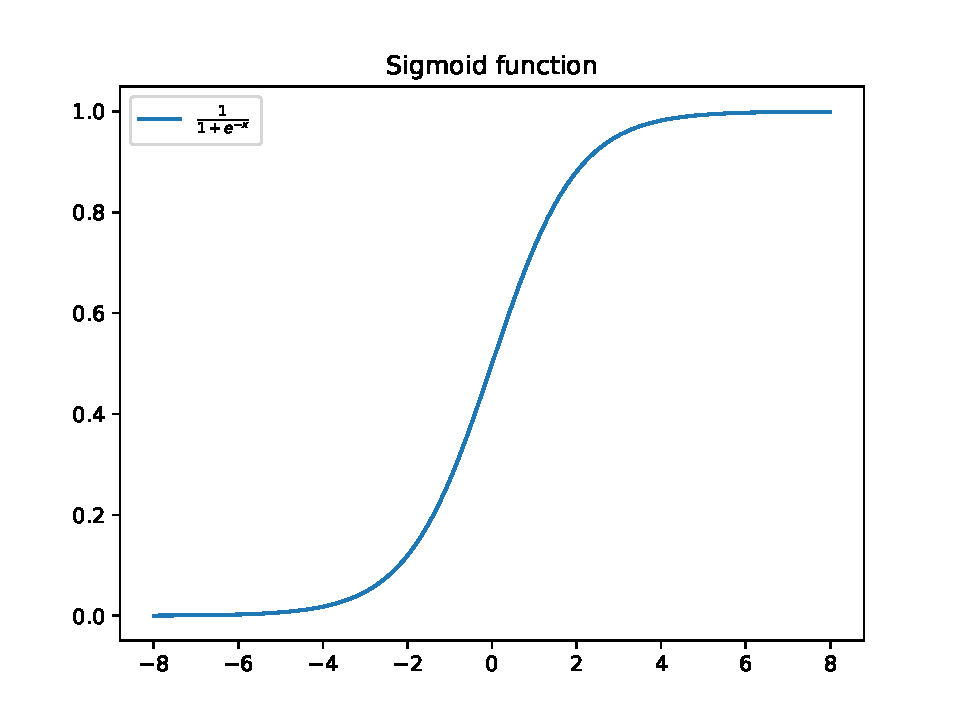
\includegraphics[width=0.55\linewidth]{sigmoid}
    \label{fig:sigmoid}
\end{figure}

1] Show that $\sigma$ is differentiable and that 

\begin{equation}
    \forall z, \sigma'(z) = \sigma(z)\sigma(-z)
\end{equation}

2] Show that $l( \hat{y}, y)$ is strictly convex in its first argument, which means for fixed $y$, $ \hat{y}\mapsto l( \hat{y},y)$ is strictly convex. Using properties that relate convexity and the derivative of a function, and using the sigmoid function will be helpful.
\\

3] Without regularization, the empirical risk writes:

\begin{equation}
    R_n(\theta)=\frac{1}{n} \sum^{n}_{i=1} l(x_i^T\theta, y_i)
\end{equation}

\begin{itemize}
    \item[\textbf{a}] Show that $\theta \rightarrow R_n(\theta)$ is convex
    \item[\textbf{b}] Compute the gradient $\nabla_{\theta}R_n(\theta)$ of the empirical risk $R_n(\theta)$ in this setting.
\end{itemize}


\end{document}
